\chapter{The FACT Open Crab Sample}
%
This analysis is exclusively using openly accessible data \cite{fact-data}. In November 2017 the
FACT collaboration made a dataset of Crab Nebula observations public
\cite{FACT-Design, FACT-Calib}. This dataset contains $\SI{17.7}{\hour}$
of Crab Nebula observations made between November 1, 2013 and November 6, 2013.
This sample is chosen because of the good observation conditions. Alongside the
data Monte Carlo simulations (MC) for diffuse proton air-showers and point-like
as well as diffuse gamma ray air-showers are distributed. The observations
cover a zenith distance between $\SIrange{6}{30}{\degree}$, \autoref{fig:zenith}.
%
\begin{figure}
  \centering%
  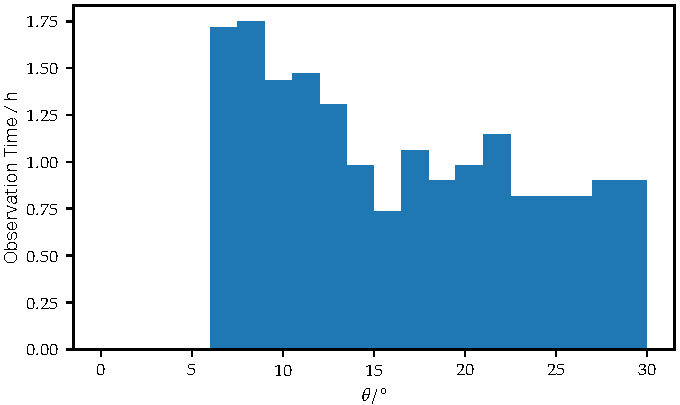
\includegraphics[width=0.8\textwidth]{Plots/zenith.pdf}%
  \caption{The distribution of the $\SI{17.7}{\hour}$ of Crab observations within the FACT open data sample over the zenith distance \cite{fact-data}.}%
  \label{fig:zenith}%
\end{figure}
%
The simulated data represents Monte Carlo simulations of air-showers
originating from protons and photons. The data sets contain events from
simulated point sources and diffuse background sources. To train the analysis
tools, dedicated truths for each of the tasks are needed. The simulations
contain these truths, and are used for this task. Therefore, the quality of
these simulations is essential to the quality of the analysis. The simulations
are processed in two steps: firstly the interactions of cosmic rays with earth's
atmosphere is computed and secondly, the interaction of the generated Cherenkov
light with the telescopes hardware is simulated. The interaction of the particles with the atmosphere and the resulting air-showers are simulated by the framework CORSIKA~\cite{CORSIKA}.

The detector response of FACT's camera, including
triggers, is then determined for the simulated events using CERES~\cite{ceres}.

The parameters used for generating the simulations are shown below.

\begin{table}
  \centering%
  \begin{tabular}{l
                  c
                  c}
      \toprule
      {}    & Gammas  & Protons      \\
      \midrule
      Energy Range & \SI{200}{\GeV} – \SI{50}{\TeV} & \SI{100}{\GeV} – \SI{200}{\TeV} \\
      Spectral Slope & \num{-2.7} & \num{-2.7} \\
      Max. Impact & \SI{270}{\meter} & \SI{400}{\meter} \\
      Zenith Distance & \ang{0} – \ang{30} & \ang{0} – \ang{30} \\
      CORSIKA Events & \num{12000000} & \num{780046520}\\
      Triggered Events & \num{1914812} & \num{509652}\\
      \bottomrule
  \end{tabular}
  \caption{Parameters and number of events regarding the MC simulated events.}
  \label{tab:mcs}
\end{table}

\section{FACT-Tools Open Crab Analysis}\label{sec:facttools}
%
The FACT open data sample's LP representation has been analyzed, using the
classical analysis methods \cite{openana}. The data is processed, cleaned and parametrized via the framework FACT-Tools~\cite{facttools}. The data set contains the same observations and MC simulations as the PhotonStream data set, but in LP representation.

As described in \autoref{fig:analysis}, the analysis uses the pixel-based
cleaning algorithm, as defined in \autoref{sec:thresh}. Furthermore, the
parameter set, used for the analysis tasks, contains a number of additional
features, not yet implemented in the
\texttt{FeatureStream}~\cite{FeatureStream}. In contrast to this work, the
quality cuts on the used events were optimized and are based on the work and
experience of hitherto performed analyses. The three main tasks of such
analyses (gamma-hadron separation, energy reconstruction, origin
reconstrcution) are performed with the machine learning package \texttt{iact-tools}, based on \texttt{scikit-learn}, as described in \autoref{ch:analysis}.
The analysis tasks, therefore, are performed the same way as for the
PhotonStream analysis, but with a parameter set beyond the standard features implemented for the PhotonStream analysis.

For the above mentioned reasons concerning the data representation and anylsis
details, a direct comparison of results is very hard. The results of this
classical analysis are nevertheless based on the same data and definetely allow
for a comparison of the PhotonStream's characteristics to LP data. They
furthermore show the currently possible performance and therefore set the reference of FACT analysis on a dataset of the size and quality as this one.
